\section{Mathematical Results on Modified Piccoli Model}
\subsection{Cauchy Problem}
%\subsubsection{Cauchy Problem}
\begin{frame}[fragile]
\frametitle{Cauchy Problem}
Consider a junction with one incoming mainline modeled by the real interval $]-\infty,0]$ and an outgoing mainline modeled by the interval $[0,+\infty[$, one onramp and one offramp. 
\begin{equation}
	\label{eq:CP}
		\left\{
		\begin{array}{ll}
		\del_t \rho_i + \del_x f_i(\rho_i) =0, & (t,x)\in\R^+\times I_i, \\
		\dfrac{dl(t)}{dt}=D_i(t)-r_i(t), & t\in\R^+ ,\\
		\rho_i(0,x)=\rho_{i,0}(x), & \text{on } I_i \\
		l(0)=l_0.
		\end{array}
		\right.
\end{equation}
Coupled with the following junction problem
\begin{eqnarray}
 	\label{eq:JunctionProblem}
		&d(t)&=\left\{
			 \begin{array}{ll}
			 r^{\max}_i &\hbox{if}~l(t)>0 , \\ 
			 \min{(D_i(t), r^{\max}_i)} &\hbox{if}~l(t)=0,
			 \end{array}
			 \right.\\ \nonumber
		&\delta(t)&=\min{(f^{\max},v\rho_i)},	 \\ \nonumber
		&\sigma(t)&=\min{(f^{\max},w(\rho_{i+1} - \rho_{max}))},\\ \nonumber
		&r_{i+1}(t)&=\beta f^{\text{out}}_i(\rho_i(t,0-)),	\\ \nonumber	
		&f^{\text{in}}_{i+1}(\rho_{i+1}(t,0+))&=\min{((1-\beta)\delta(t)+d(t), \sigma(t))}.
\end{eqnarray}

\end{frame}

%\subsubsection{Solution}
\begin{frame}[fragile]
\frametitle{Solution}
\begin{definition}
	\label{def:weak_sol}
	A collection of functions $(\rho_1,\rho_2,l)\in \prod_{i=1}^2 \CC^0\left( \R^+; \L1\cap\BV (\R)\right) \times \mathbf{W^{1,\infty}}(\R^+;\R^+)$ is a solution at $J$ to (\ref{eq:CP}) if
	\begin{enumerate}%[label=(\roman{*}),ref=(\roman{*})]
		\item \label{item:i} $\rho_1$,$\rho_2$ are weak solutions on $I_1$, $I_2$, i.e.,\begin{equation}	
		\Big(\int_{\R^+}\int_{I_i}\Big( \rho_i \del_t\varphi_i +f(\rho_i)\del_x\varphi_i \Big)dxdt\Big)=0 \quad i=1,2,  		
		\label{eq:weakSolRho}
	\end{equation}
	for every $\varphi_i \in \CC^1_c(\R^+\times I_i)$. 
		%\item \label{item:ii} $f_1(\rho(t,0-))=\dfrac{P}{1-P}\gamma_{r1}$ with $P \in ]0,1[$ the priority factor;
		\item \label{item:iii} $f^{\text{out}}_{i}(\rho_{i}(t,0-))+r_i(t)=f^{\text{in}}_{i+1}(\rho_{i+1}(t,0+))+r_{i+1}(t)$; 
		\item \label{item:iv} minimize $dist\left(\mathbf{f}, P \right)$ such that $f^{\text{in}}_{i+1}(\rho_{i+1}(t,0+))$ is maximized; %subject to \ref{item:ii},\ref{item:iii} and \eqref{eq:JunctionProblem};
		\item \label{item:v} $l$ is a solution of the ODE  for a.e. $t\in\R^+$.		
	\end{enumerate}
\end{definition}

\end{frame}

\subsection{Existence Theorem}
%\subsubsection{Main theorem}
\begin{frame}[fragile]
\frametitle{Main Theorem}
If we consider one junction with one incoming mainline modeled by the real interval $]-\infty,0]$ and an outgoing mainline modeled by the interval $[0,+\infty[$, one onramp and one offramp it holds: 
\vspace*{5mm}
\begin{theorem}
	\label{th:existenceSol}
	Consider a junction $J$ and fix a priority parameter $P \in  ]0,1[$. For every $\rho_{1,0}$,$\rho_{2,0} \in [0,1]$ and $l_0 \in [0, +\infty]$, there exists a unique admissible solution $(\rho_1(t,x),\rho_2(t,x),l(t))$ in the sense of Definition \ref{def:weak_sol} such that for a.e. $t>0$ it holds
$$(\rho_1(t,0-),\rho_2(t,0+))=\RS_{l(t)}(\rho_1(t,0-),\rho_2(t,0+)).$$ 
\end{theorem}
\end{frame}

%\subsubsection{Solution of the Riemann Solver}
\begin{frame}
	\frametitle{Solution of $\RS$}
	\begin{figure}[ht]
\centering
\begin{tikzpicture}[scale=0.8]
	\draw[<-] (0,6) -- (0,0);
	\draw[->] (-6,0) -- (6,0);	
	\draw (0,0) -- (2,2)--(6,6);
	\draw (0,0) -- (-2,2)--(-6,6);
	\draw (0,3) -- (2,6);
	\node (left) at (-0.2,3.1) {$\bar{t}$};	
	\node (left) at (-0.2,5.85) {$t$};
	\node (below) at (5.9,-0.3) {$x$};
	\node (below) at (0,-0.3) {$0$};
	\node (above) at (-3,1) {$\rho_{1,0}$};
	\node (above) at (3,1) {$\rho_{2,0}$};
	\node (above) at (-3,4) {$\hat{\rho}_1$};
	\node (above) at (3,4) {$\hat{\rho}_2$};
	\node (above) at (0.5,5) {$\bar{\rho}_2$};
\end{tikzpicture}

%\caption{Generic 2x2 junction.}
\label{fig:RiemProb}
\end{figure}
\end{frame}

%\subsubsection{Proof I}
\begin{frame}[fragile]
	\frametitle{Properties of the $\Riem$}
Define $\gamma_{1,t}=f^{\text{out}}_i(\rho(t,0-))$, $\gamma_{2,t}=f^{\text{in}}_{i+1}(\rho(t,0+))$, $\gamma_{r,t}=r_i(t)$ and $\gamma^{\max}_{1,t}=\delta(t)$, $\gamma^{\max}_{2,t}=\sigma(t)$, $\gamma^{\max}_{r,t}=d(t)$. \\
\vspace*{2mm}
\textbf{Some Properties of the Riemann Solver:}\\
	\begin{itemize}
	\item<1-> $\gamma_{i,t_{0}}=\gamma^{\max}_{i,t_{0}} \Rightarrow \gamma^{\max}_{i,t_{0}+}=\gamma^{\max}_{i,t_{0}}$ $\forall i=1,2,r$. \\ \vspace*{2mm} This holds because of the definitions of the functions $\tau(\rho)$, $\delta(t)$ and $\sigma(t)$ for the mainlines and the definition of $d(t)$ for the ramp.
	
	\item[]{\begin{columns}
	\column{0.5 \textwidth}
	\begin{figure}[ht]
\centering
{
\resizebox{.7\columnwidth}{!}{
\input{propertyInc1}}
\caption{Incoming road.}
\label{fig:PI1}}
\end{figure}
	\column{0.5 \textwidth}
	\begin{figure}[ht]
\centering
{
\resizebox{.7\columnwidth}{!}{
\input{propertyOut2}}
\caption{Outgoing road.}
\label{fig:PO2}}
\end{figure}
\end{columns}}
\item[]{ For the ramp: $D>r^{\max}=\gamma_{r,t_{0}}^{\max} \Rightarrow \gamma_{r,t_{0}}^{\max}=\min\left(D,r^{\max}\right)=r^{\max}=\gamma_{r,t_{0}+}^{\max}.$}
\end{itemize}
\end{frame}

%\subsubsection{Proof II}
\begin{frame}[fragile]
	\frametitle{Properties of the $\Riem$ II}
\begin{itemize}
	
	\item<1-> $\gamma_{i,t_{0}}<\gamma^{\max}_{i,t_{0}} \Rightarrow \gamma^{\max}_{i,t_{0}}\leq\gamma^{\max}_{i,t_{0}+}$ $\forall i=1,2,r$. \\ \vspace*{3mm} This holds because of the definitions of $\tau(\rho)$, $\delta(t)$, $\sigma(t)$ for the mainlines and the definition of $d(t)$ for the ramp.\\
	\item[] {\begin{columns}
	\column{0.5 \textwidth}
	\begin{figure}[ht]
\centering
{
\resizebox{.9\columnwidth}{!}{
\input{propertyInc2}}
\caption{Incoming road.}
\label{fig:PI2}}
\end{figure}
	\column{0.5 \textwidth}
	\begin{figure}[ht]
\centering
{
\resizebox{.9\columnwidth}{!}{
\input{propertyOut1}}
\caption{Outgoing road.}
\label{fig:PO1}}
\end{figure}
\end{columns}}
\item[]{ For the ramp: $\forall D,r^{\max}:r^{\max}\ge\min\left(D,r^{\max}\right).$}
	\end{itemize}
\end{frame}	

%\subsubsection{Proof III}
\begin{frame}[fragile]
	\frametitle{Properties of the $\Riem$ III}
	\begin{itemize}
		\item If the solution at time $t_0$ lies on a limiting side then the solution at time $t_0+$ will lie there too.
		\vspace*{3mm}
		\item The limiting side does not change.\\ At time $t_0+$ the non limiting side can only increase while the limiting side's feasible set remains the same.
	\end{itemize}
\end{frame}
\subsubsection*{Proof IV}
\begin{frame}
	\frametitle{Sketch of the proof of self-similarity}
	\textbf{Sketch of the proof:}\\
	\begin{columns}
	\column{0.33 \textwidth}
	\begin{figure}[ht]
\centering
{
\resizebox{.9\columnwidth}{!}{
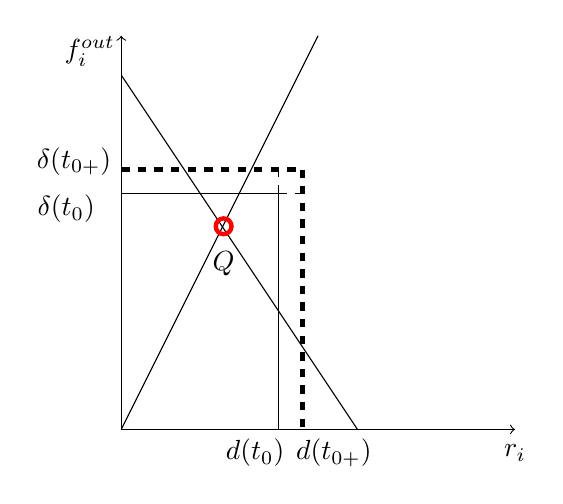
\begin{tikzpicture}
	\draw[<->] (0,5) -- (0,0) --(5,0);
	\draw (0,0) rectangle (2,3);
	%\draw [dashed](0,0) rectangle (2.3,3.3);
	\draw [dashed, ultra thick](0,3.3) -- (2.3,3.3);
	\draw [dashed, ultra thick](2.3,3.3) -- (2.3,0);
	\draw (3,0) -- (0,4.5);
	\draw [dashed](2,3) -- (2.3,3);
	\draw [dashed](2,3) -- (2,3.3);
	%\draw[fill=gray] (0,0)--(0,3) to (0,0) -- (2,0) to (2,0)--(2,1.5) to (2, 1.5)--(1,3) to (0.58,3)--(0,3) ;
	\draw (0,0) -- (1,2)--(2.5,5);
	\draw[ultra thick, red](1.3,2.58) circle (0.1);
	\node (below) at (5,-0.3) {$r_i$};
	\node (below) at (1.7,-0.3) {$d(t_{0})$};
	\node (below) at (2.7,-0.3) {$d(t_{0+})$};
	\node (left) at (-0.4,4.8) {$f^{\text{out}}_{i}$};
	\node (left) at (-0.7,2.8) {$\delta(t_{0})$};
	\node (left) at (-0.6,3.4) {$\delta(t_{0+})$};
	%\node (right) at (3.5,1.5) {$\hat{\gamma}_3=\gamma_1+\gamma_2$};
%	\node (above) at (1,1.5) {$\Omega$};
	%\node (right) at (3.2,4) {$\gamma_2=\frac{P}{1-P}\gamma_1$};
	\node (below) at (1.3,2.1) {$Q$};
\end{tikzpicture}}
%\caption{Solution of the Riemann Problem.}
\label{fig:SS1}}
\end{figure}
	\column{0.33 \textwidth}
	\begin{figure}[ht]
\centering
{
\resizebox{1\columnwidth}{!}{
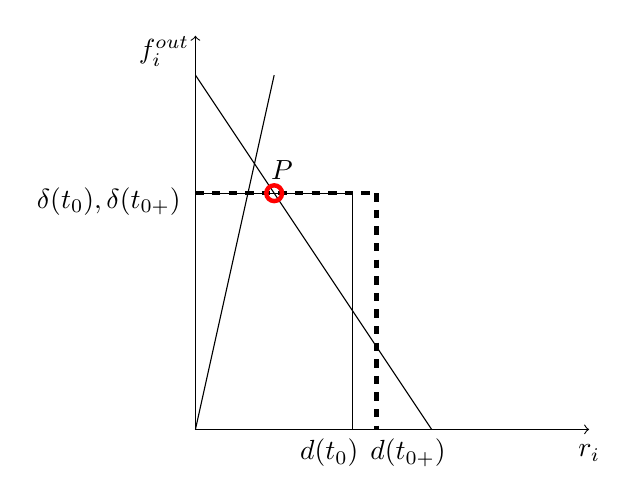
\begin{tikzpicture}
	\draw[<->] (0,5) -- (0,0) --(5,0);
	\draw (0,0) rectangle (2,3);
	\draw (3,0) -- (0,4.5);
	\draw [dashed, ultra thick](2.3,3) -- (2.3,0);
	\draw [dashed, ultra thick](0,3) -- (2.3,3);
	%\draw[fill=gray] (0,0)--(0,3) to (0,0) -- (2,0) to (2,0)--(2,1.5) to (2, 1.5)--(1,3) to (0.58,3)--(0,3) ;
	\draw (0,0) -- (1,4.5);
	\draw[ultra thick, red](1,3) circle (0.1);
	\node (below) at (5,-0.3) {$r_i$};
	\node (below) at (1.7,-0.3) {$d(t_{0})$};
	\node (below) at (2.7,-0.3) {$d(t_{0+})$};
	\node (left) at (-0.4,4.8) {$f^{\text{out}}_i$};
	%\node (left) at (-0.4,2.8) {$}$};
	\node (left) at (-1.1,2.9) {$\delta(t_{0}), \delta({t_{0+}})$};
	%\node (right) at (3.5,1.5) {$\hat{\gamma}_3=\gamma_1+\gamma_2$};
	%\node (above) at (1,1.5) {$\Omega$};
	%\node (right) at (2.2,4) {$\gamma_2=\frac{P}{1-P}\gamma_1$};
	\node (below) at (1.1,3.3) {$P$};
\end{tikzpicture}}
%\caption{Solution of the Riemann Problem.}
\label{fig:SS2}}
\end{figure}
	\column{0.33 \textwidth}
	\begin{figure}[ht]
\centering
{
\resizebox{.9\columnwidth}{!}{
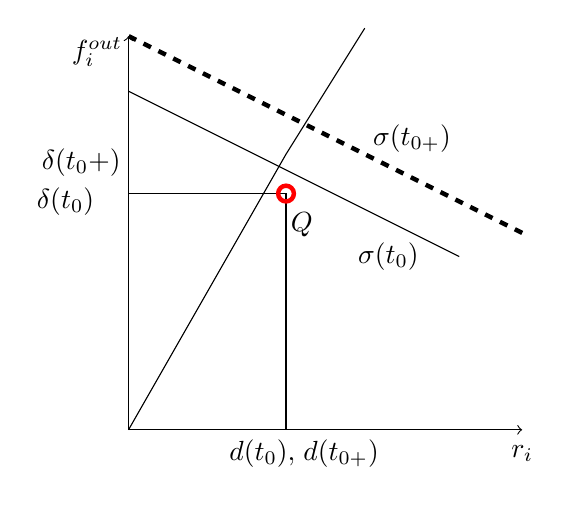
\begin{tikzpicture}
	\draw[<->] (0,5) -- (0,0) --(5,0);
	\draw (0,0) rectangle (2,3);
	%\draw [dashed](0,0) rectangle (2.3,3.3);
	%\draw [dashed, ultra thick](0,3.3) -- (2.3,3.3);
	%\draw [dashed, ultra thick](2.3,3.3) -- (2.3,0);
	\draw (4.2,2.2) -- (2.2,3.2)--(0,4.3);
	\draw [dashed, ultra thick](5,2.5) -- (2,4)--(0,5);
	%\draw [dashed](2,3) -- (2.3,3);
	%\draw [dashed](2,3) -- (2,3.3);
	%\draw[fill=gray] (0,0)--(0,3) to (0,0) -- (2,0) to (2,0)--(2,1.5) to (2, 1.5)--(1,3) to (0.58,3)--(0,3) ;
	\draw (0,0) -- (2,3.5)--(3,5.1);
	\draw[ultra thick, red](2,3) circle (0.1);
	\node (below) at (5,-0.3) {$r_i$};
	\node (below) at (1.7,-0.3) {$d(t_0),$};
	\node (below) at (2.7,-0.3) {$d(t_{0+})$};
	\node (left) at (-0.4,4.8) {$f_i^{\text{out}}$};
	\node (left) at (-0.8,2.9) {$\delta(t_0)$};
	\node (above) at (3.6,3.7) {$\sigma(t_{0+})$};
	\node (above) at (3.3,2.2) {$\sigma(t_{0})$};
	\node (left) at (-0.6,3.4) {$\delta(t_0+)$};
	%\node (right) at (3.5,1.5) {$\hat{\gamma}_3=\gamma_1+\gamma_2$};
%	\node (above) at (1,1.5) {$\Omega$};
	%\node (right) at (3.2,4) {$\gamma_2=\frac{P}{1-P}\gamma_1$};
	\node (below) at (2.2,2.6) {$Q$};
\end{tikzpicture}}
%\caption{Solution of the Riemann Problem.}
\label{fig:SS3}}
\end{figure}

\end{columns}
\end{frame}
